\chapter{Aufgabe 2: Summe von acht Zahlen}

\begin{figure}[tbp]
 \centering 
 %
 \begin{subfigure}{.33\textwidth}
  \centering 
  \fbox{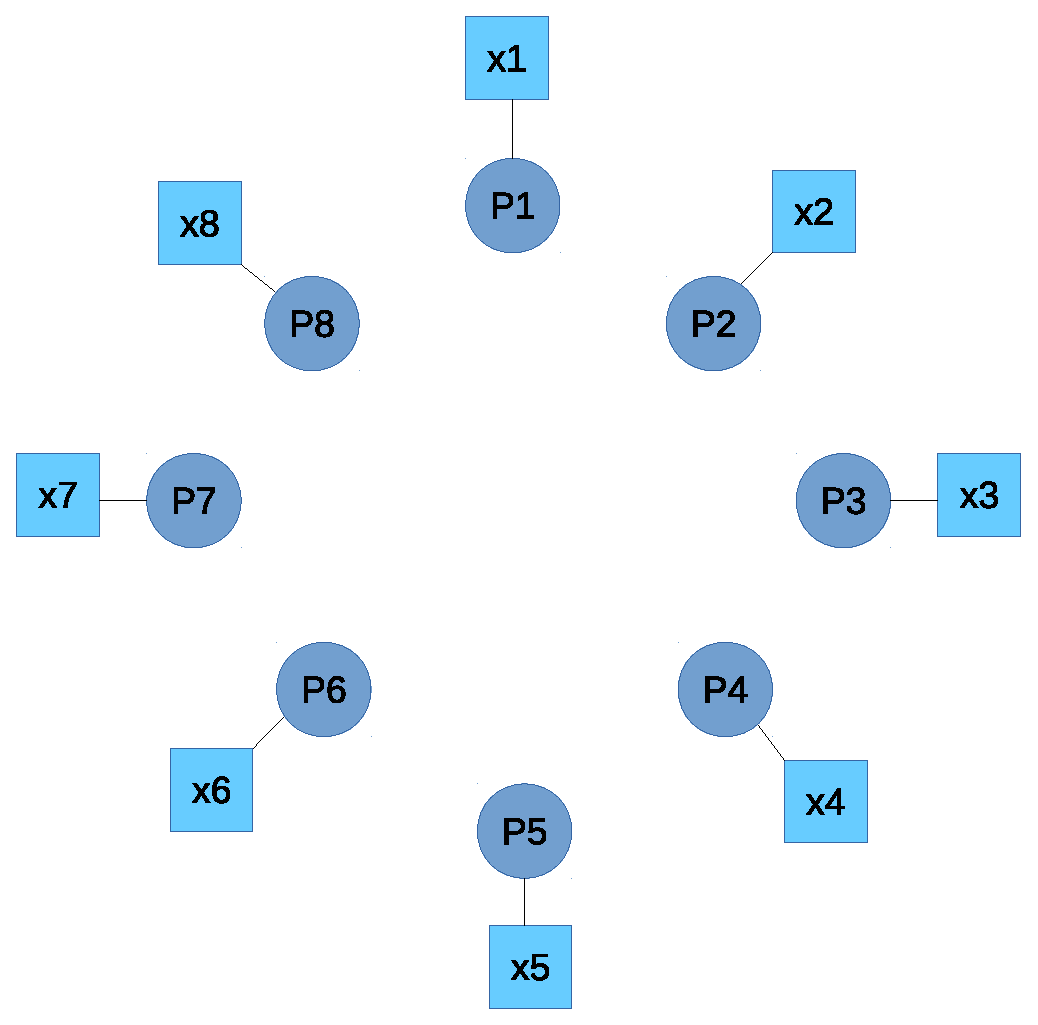
\includegraphics[width=.85\textwidth]{kreis_0.eps}}
  \caption{$t=0$.}
 \end{subfigure}
 %
 \begin{subfigure}{.33\textwidth}
  \centering 
  \fbox{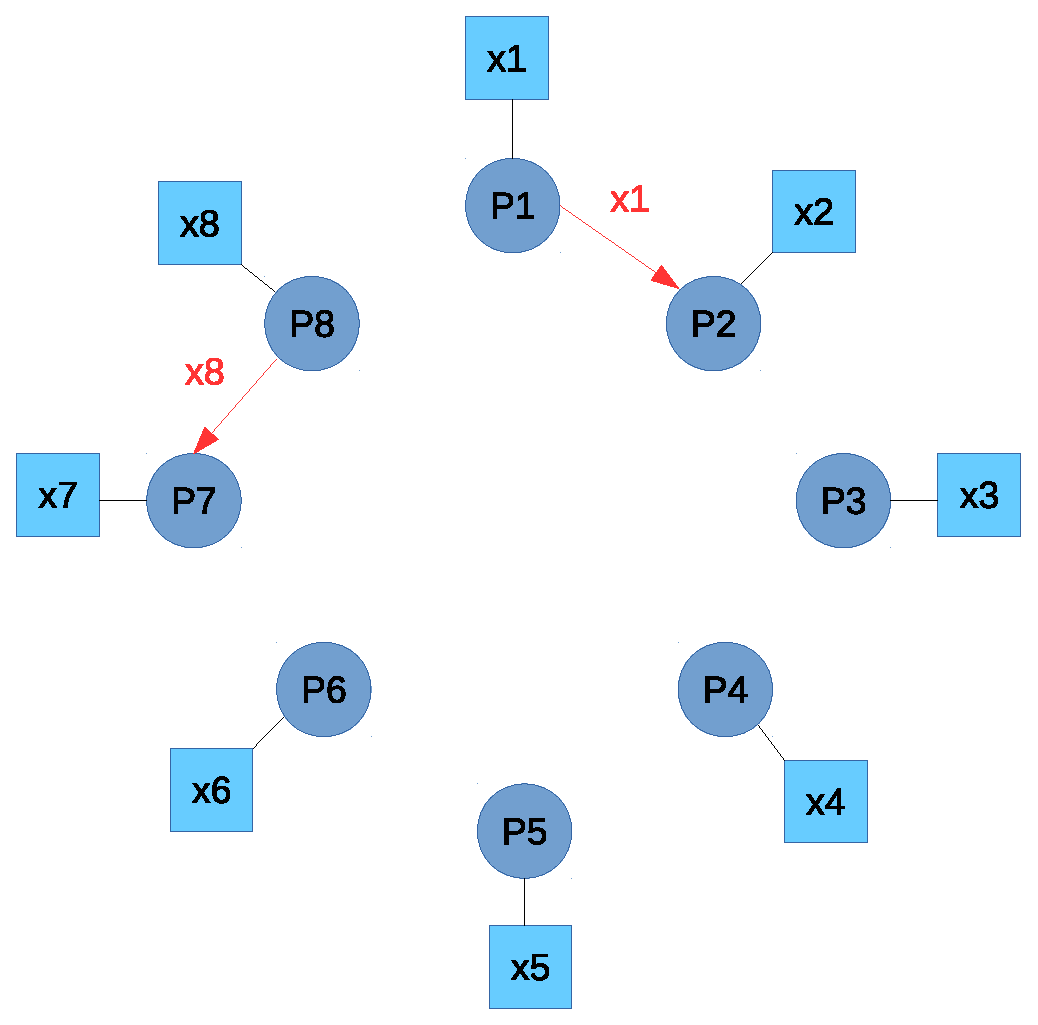
\includegraphics[width=.85\textwidth]{kreis_1.eps}}
  \caption{$t=t_c$.}
 \end{subfigure}
%
 \begin{subfigure}{.33\textwidth}
  \centering 
  \fbox{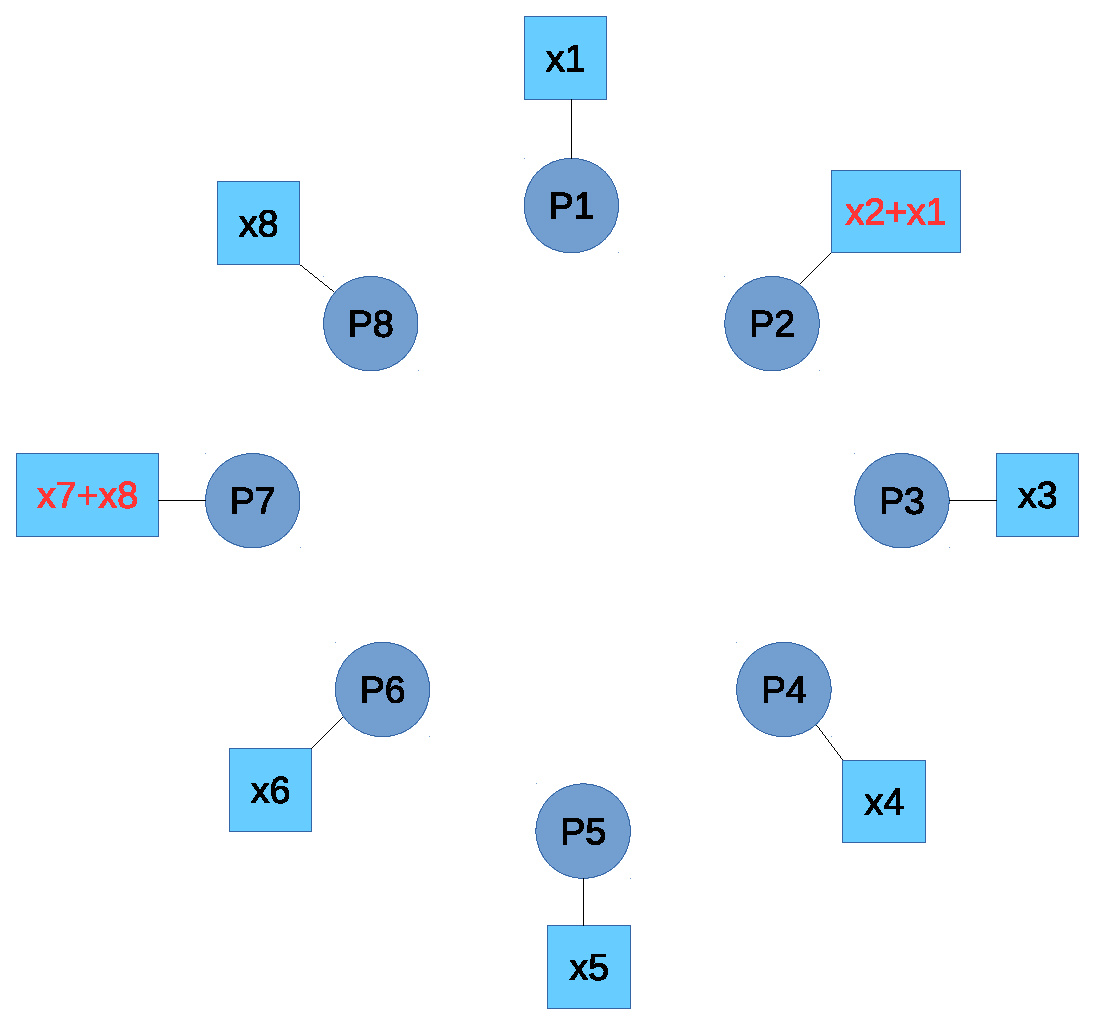
\includegraphics[width=.85\textwidth]{kreis_2.eps}}
  \caption{$t=t_c+t_a$.}
 \end{subfigure}
%
\begin{subfigure}{.33\textwidth}
  \centering 
  \fbox{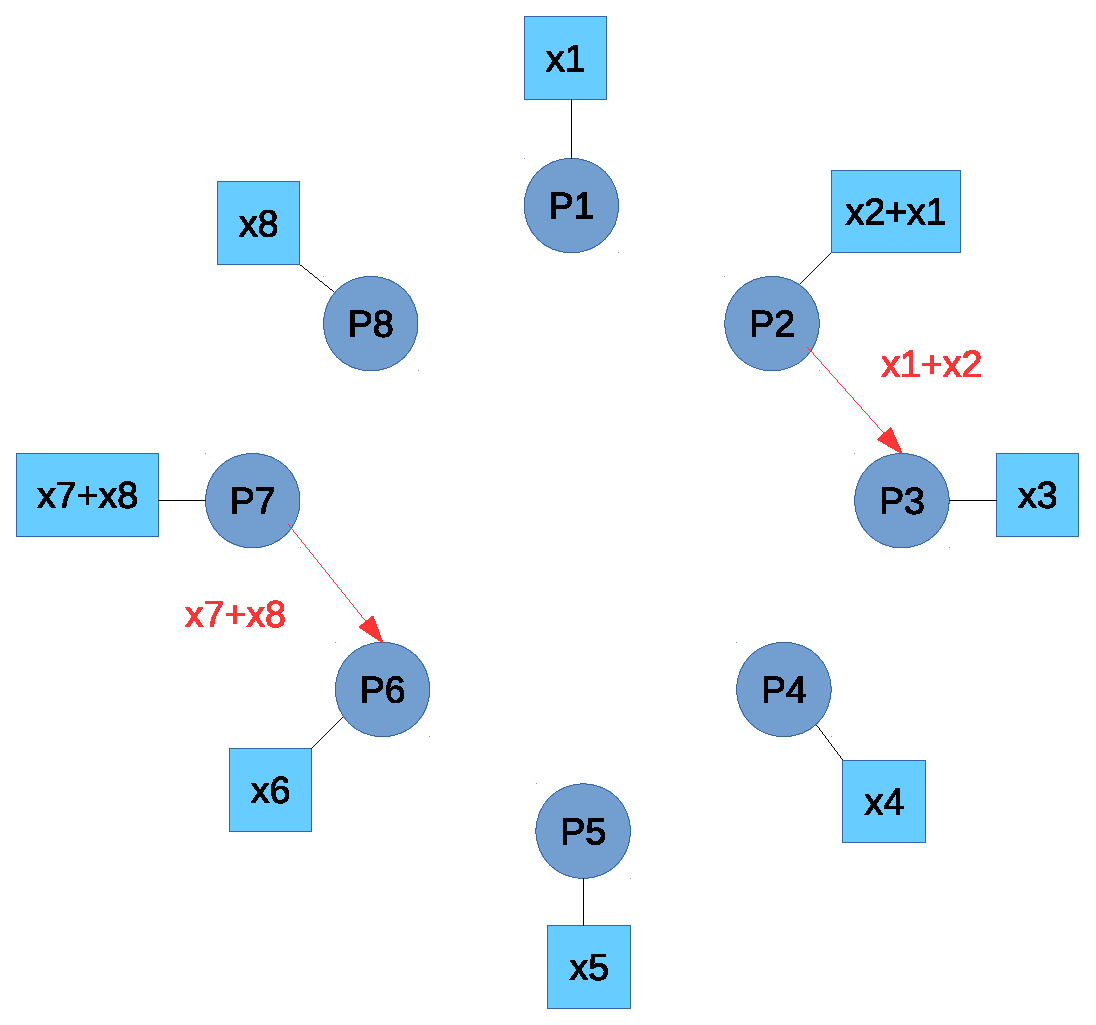
\includegraphics[width=.85\textwidth]{kreis_3.eps}}
  \caption{$t=2t_c+t_a$.}
 \end{subfigure}
%
\begin{subfigure}{.33\textwidth}
  \centering 
  \fbox{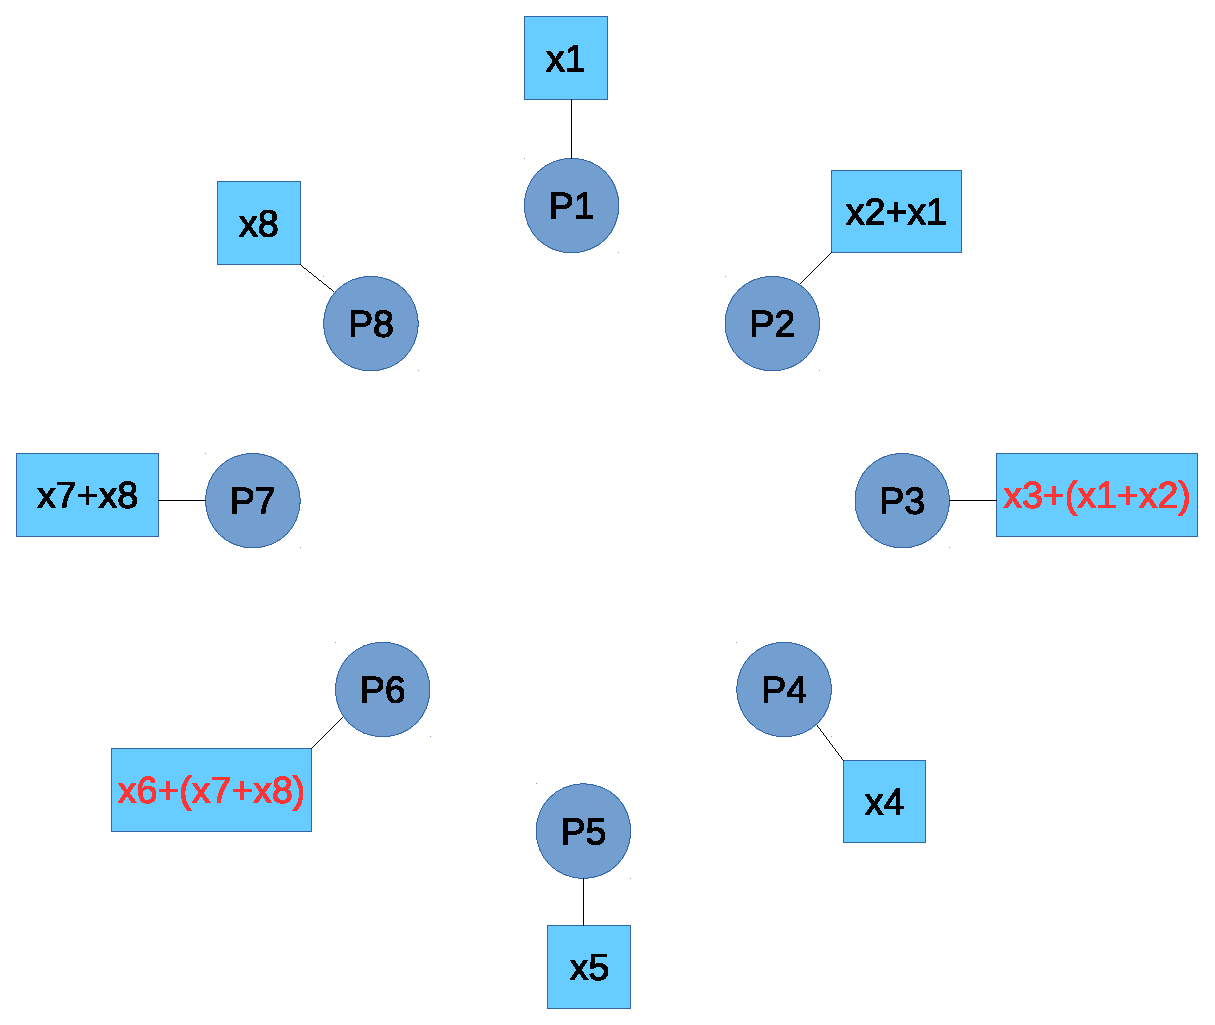
\includegraphics[width=.85\textwidth]{kreis_4.eps}}
  \caption{$t=2t_c+2t_a$.}
 \end{subfigure}
%
\begin{subfigure}{.33\textwidth}
  \centering 
  \fbox{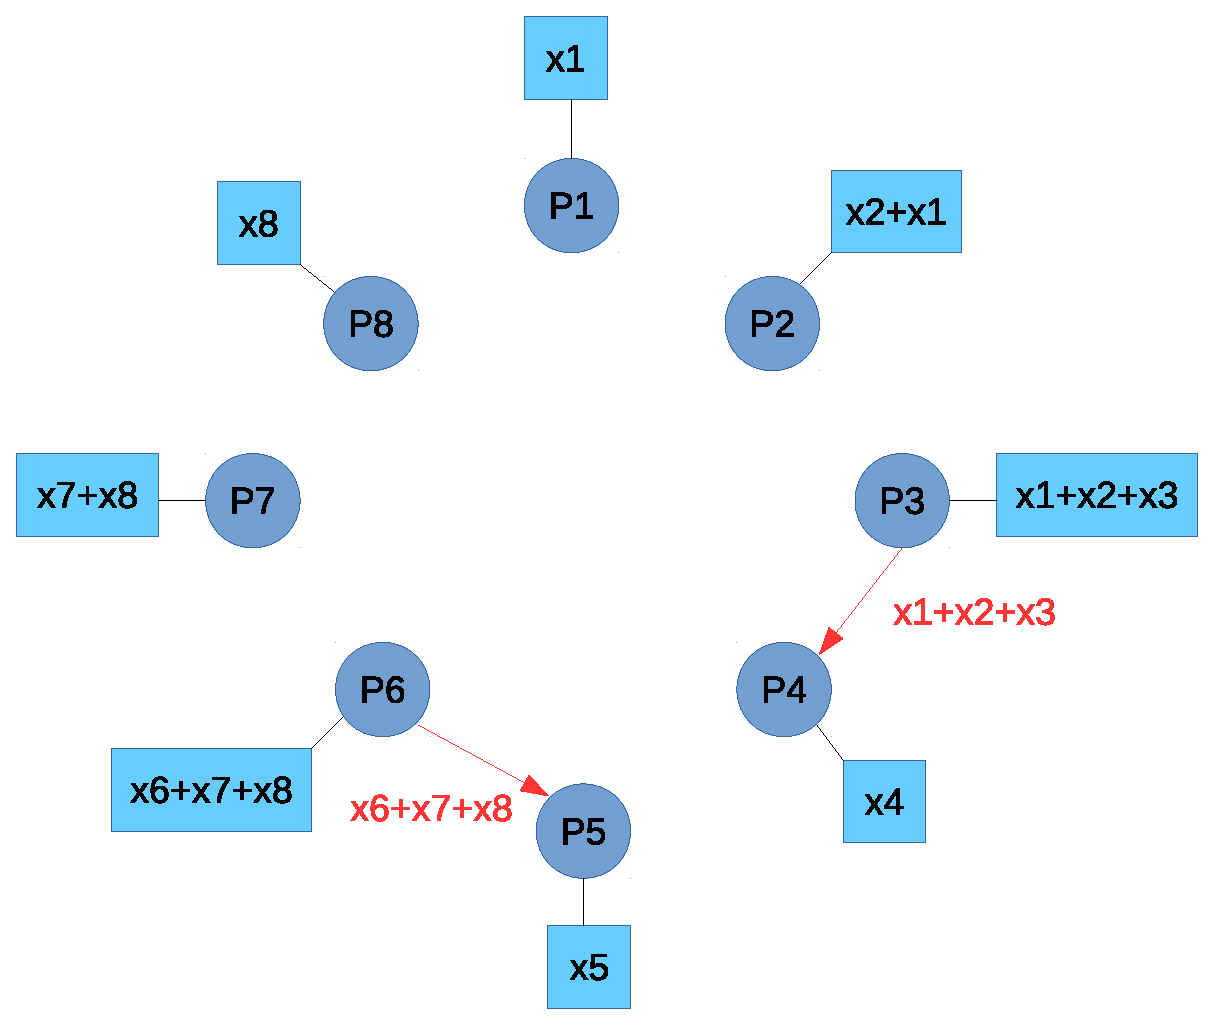
\includegraphics[width=.85\textwidth]{kreis_5.eps}}
  \caption{$t=3t_c+2t_a$.}
 \end{subfigure}
%
\begin{subfigure}{.33\textwidth}
  \centering 
  \fbox{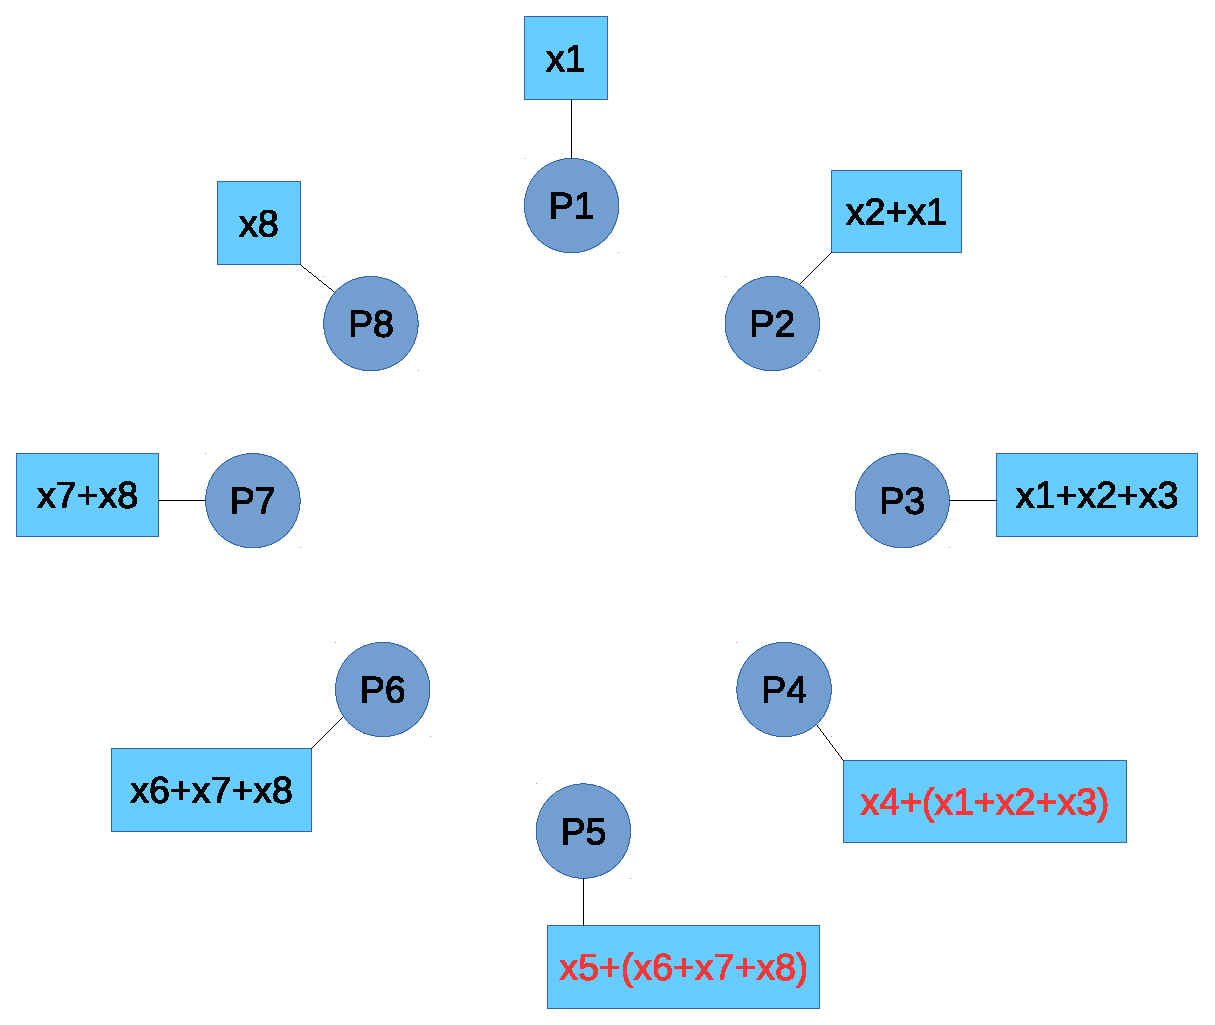
\includegraphics[width=.85\textwidth]{kreis_6.eps}}
  \caption{$t=3t_c+3t_a$.}
 \end{subfigure}
%
\begin{subfigure}{.33\textwidth}
  \centering 
  \fbox{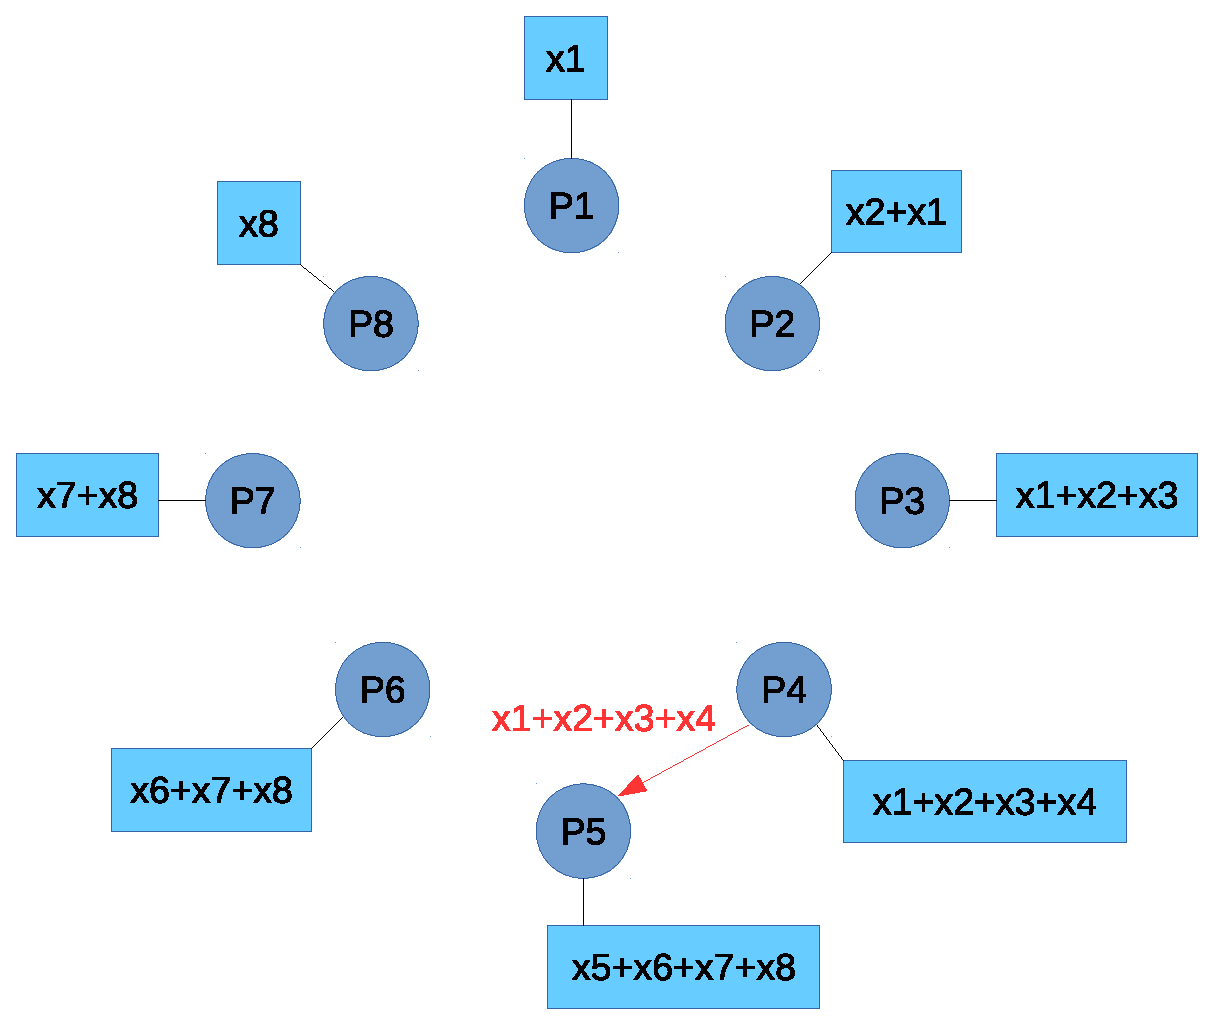
\includegraphics[width=.85\textwidth]{kreis_7.eps}}
  \caption{$t=4t_c+3t_a$.}
 \end{subfigure}
%
\begin{subfigure}{.33\textwidth}
  \centering 
  \fbox{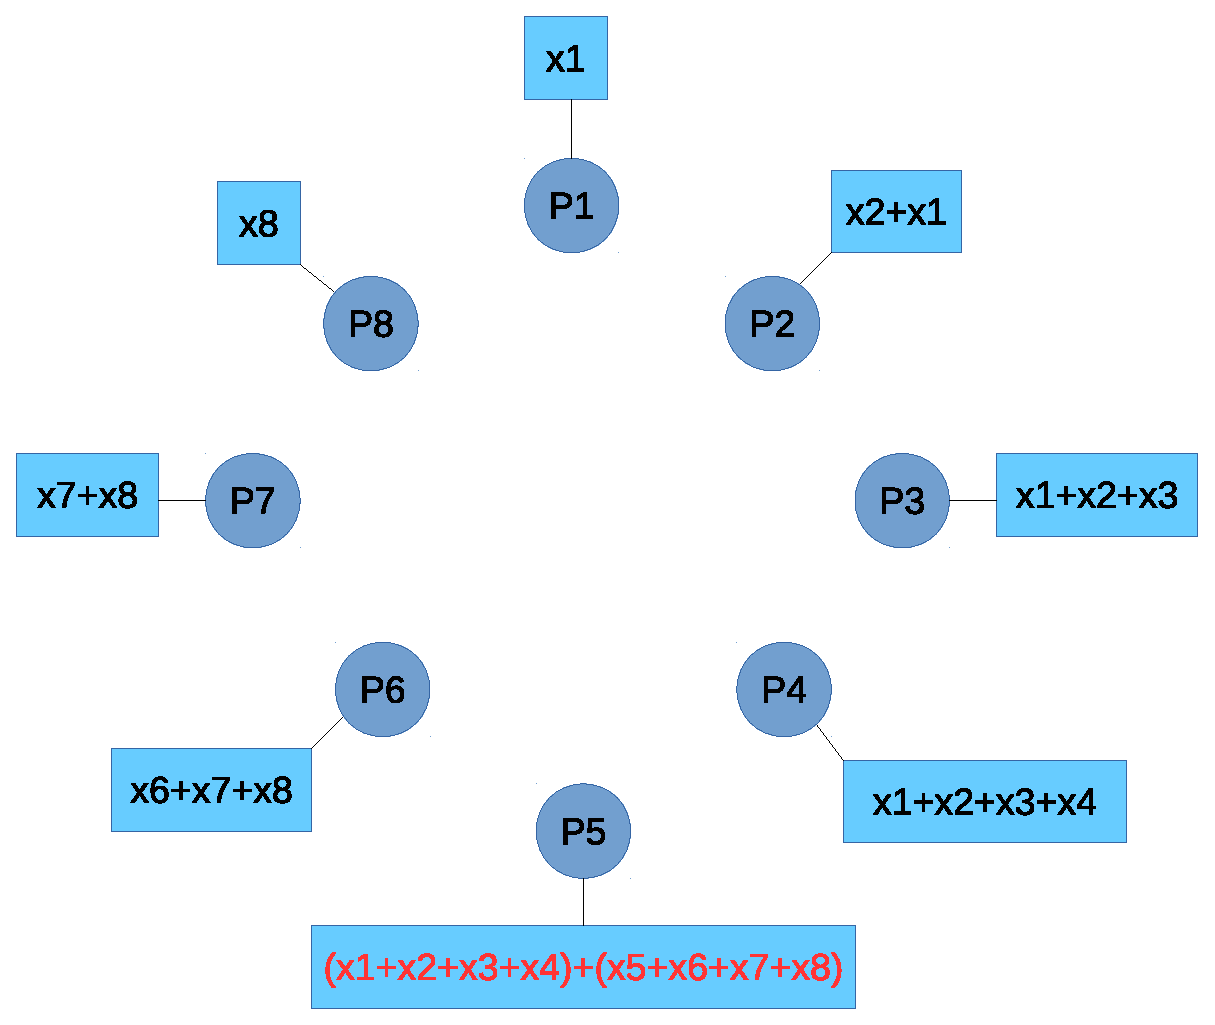
\includegraphics[width=.85\textwidth]{kreis_8.eps}}
  \caption{$t=4t_c+4t_a$.}
 \end{subfigure}
%
\caption{Veranschaulichung einer parallelen Vorgehensweise bei der Kreissitzordnung.}
\label{fig:kreis}
\end{figure}

\begin{figure}[tbp]
 \centering 
 %
\begin{subfigure}{.33\textwidth}
 \centering 
 \fbox{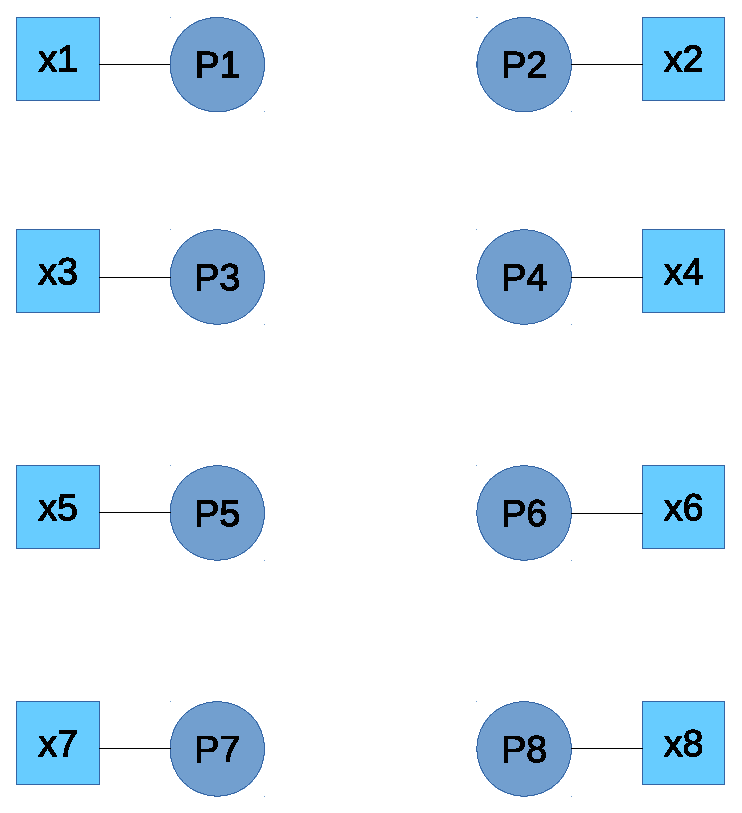
\includegraphics[width=.85\textwidth]{gitter_0.eps}}
 \caption{$t=0$.}
\end{subfigure}
%
\begin{subfigure}{.33\textwidth}
 \centering 
 \fbox{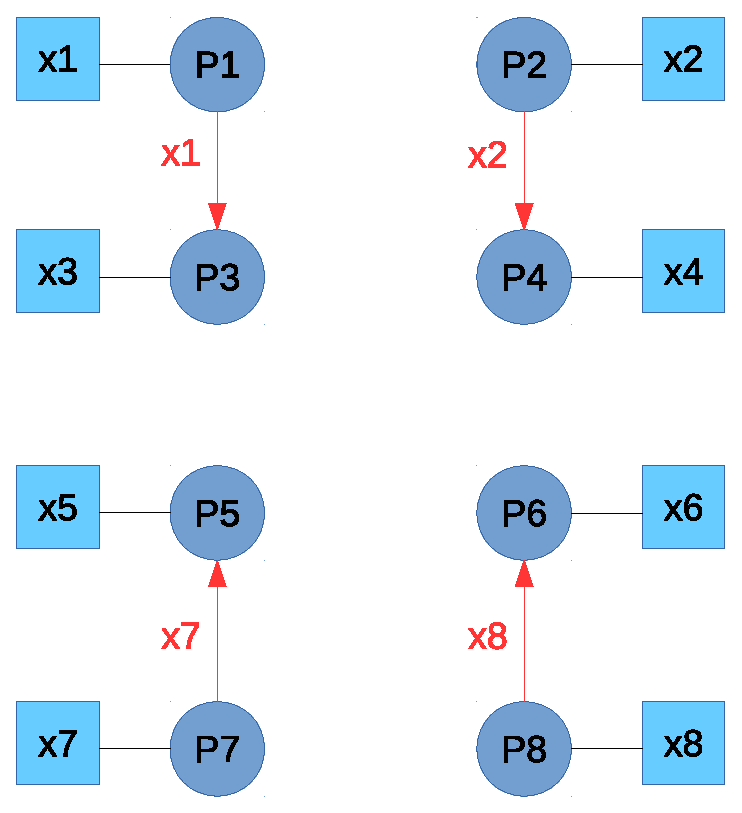
\includegraphics[width=.85\textwidth]{gitter_1.eps}}
 \caption{$t=t_c$.}
\end{subfigure}
%
\begin{subfigure}{.33\textwidth}
 \centering 
 \fbox{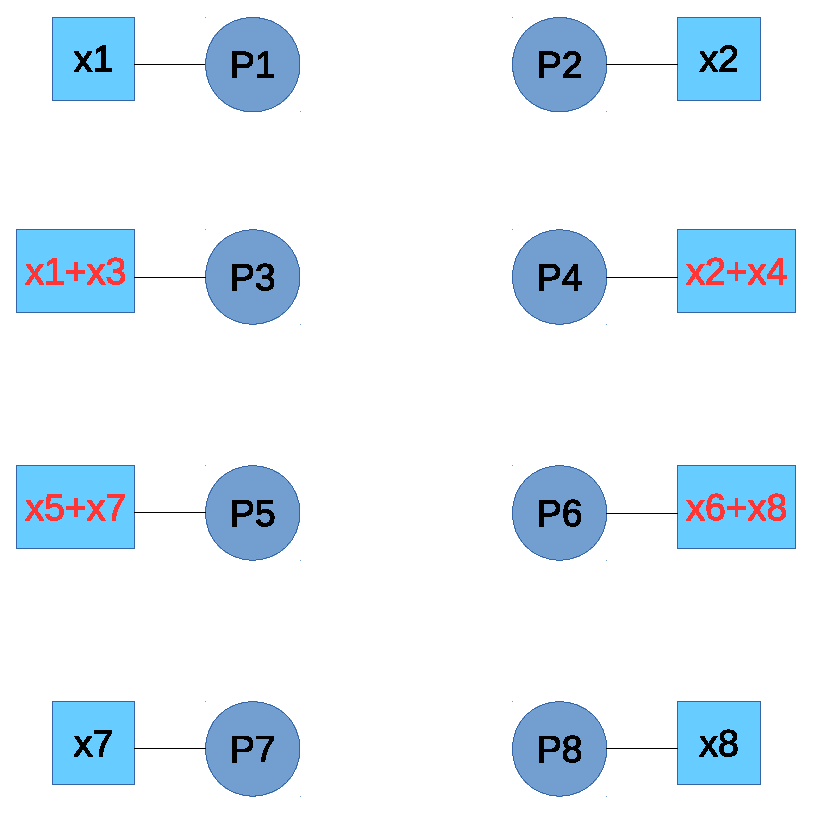
\includegraphics[width=.85\textwidth]{gitter_2.eps}}
 \caption{$t=t_c+t_a$.}
\end{subfigure}
%
\begin{subfigure}{.33\textwidth}
 \centering 
 \fbox{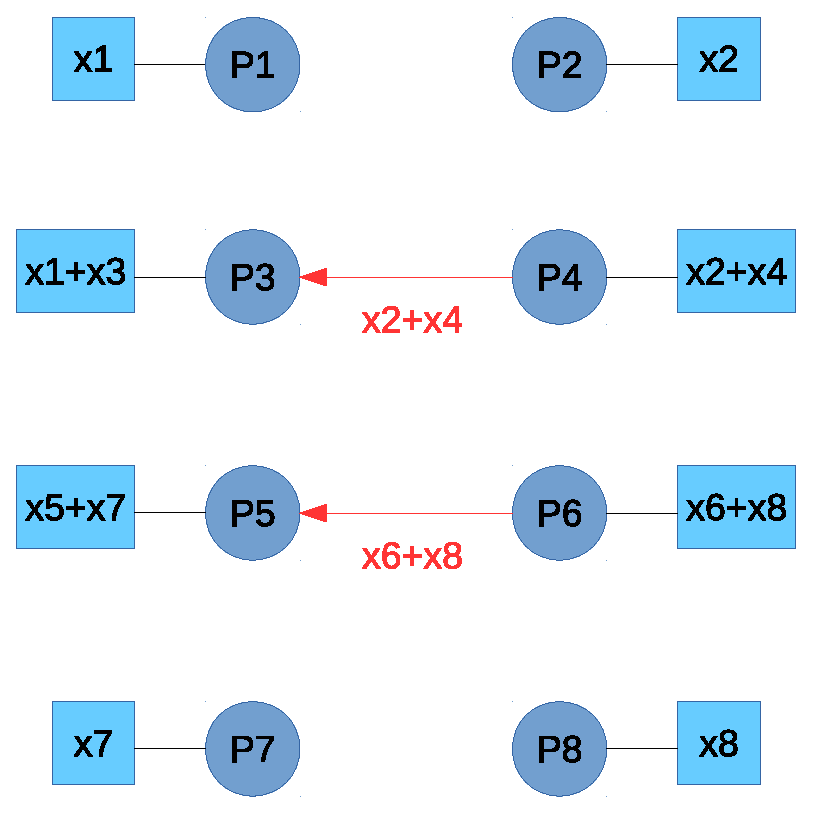
\includegraphics[width=.85\textwidth]{gitter_3.eps}}
 \caption{$t=2t_c+t_a$.}
\end{subfigure}
%
\begin{subfigure}{.33\textwidth}
 \centering 
 \fbox{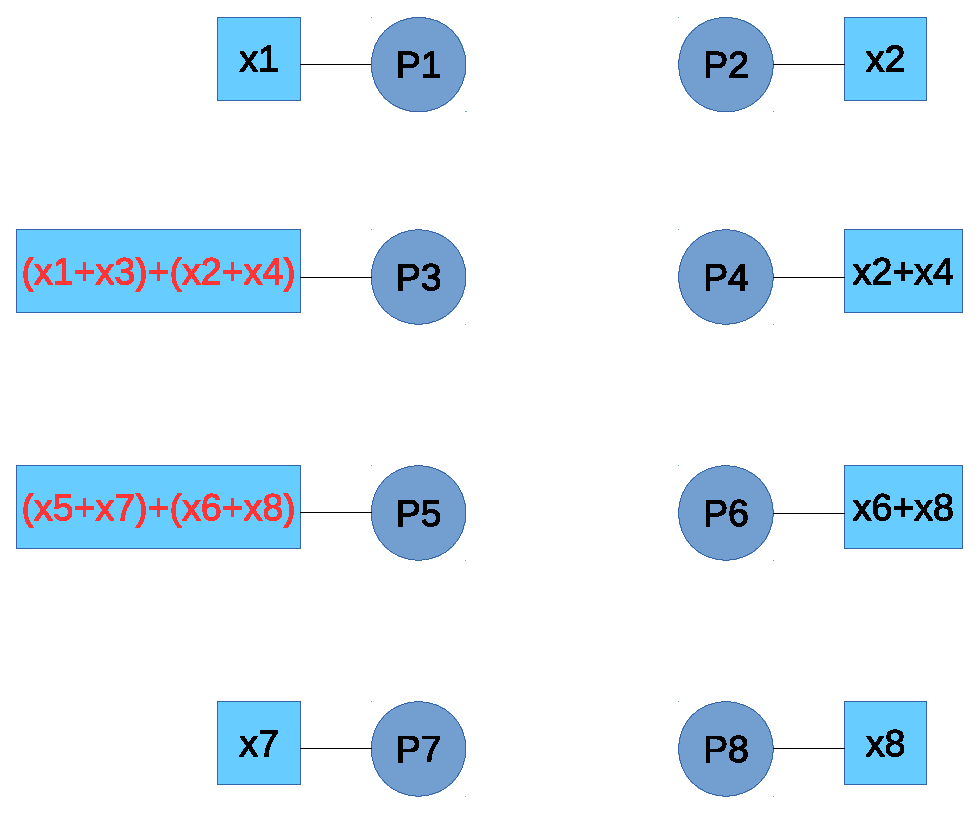
\includegraphics[width=.85\textwidth]{gitter_4.eps}}
 \caption{$t=2t_c+2t_a$.}
\end{subfigure}
%
\begin{subfigure}{.33\textwidth}
 \centering 
 \fbox{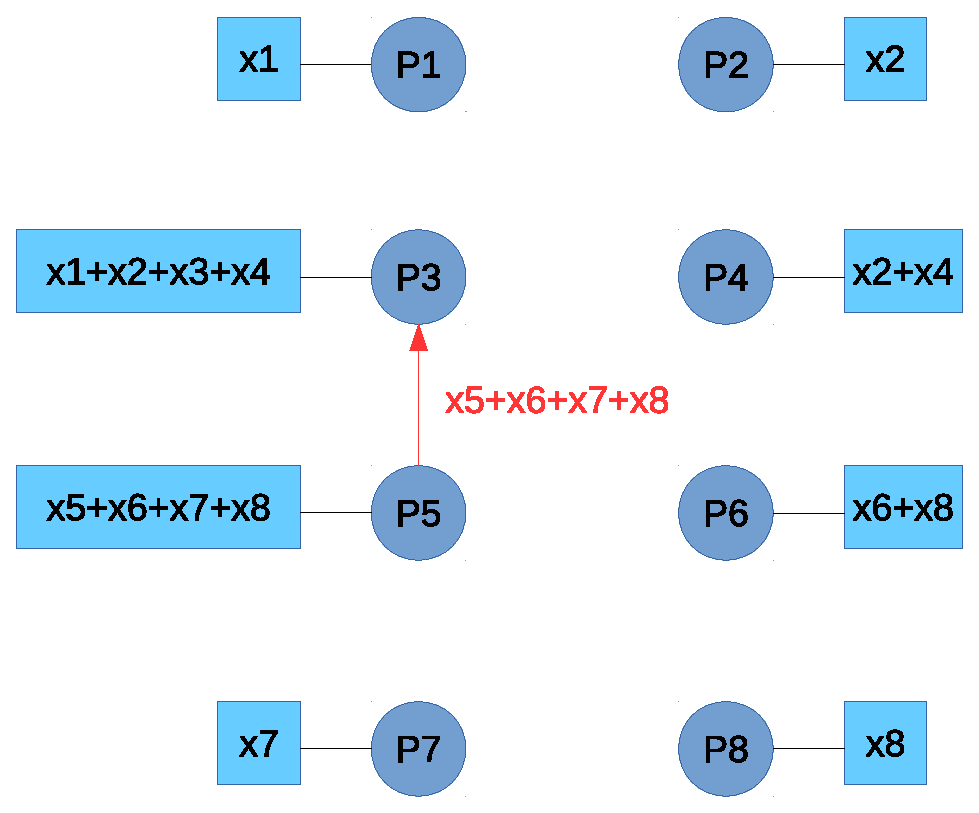
\includegraphics[width=.85\textwidth]{gitter_5.eps}}
 \caption{$t=3t_c+2t_a$.}
\end{subfigure}
%
\begin{subfigure}{.33\textwidth}
 \centering 
 \fbox{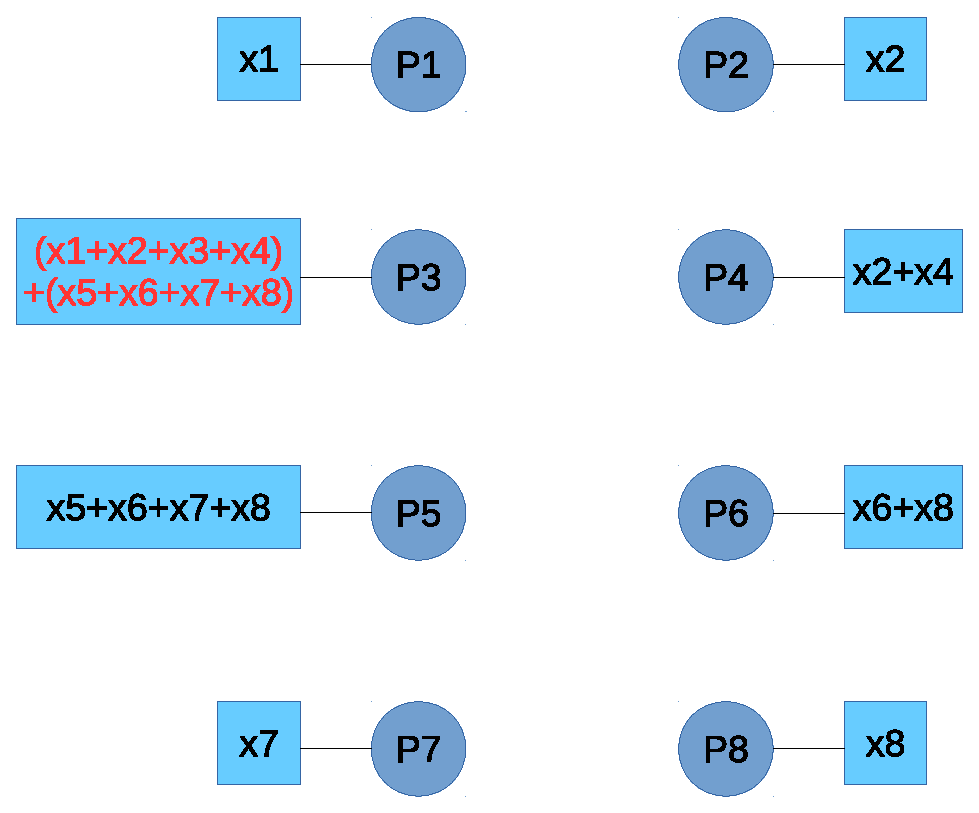
\includegraphics[width=.85\textwidth]{gitter_6.eps}}
 \caption{$t=3t_c+3t_a$.}
\end{subfigure}
%
\caption{Veranschaulichung einer parallelen Vorgehensweise bei einer $4\times2$ Gittersitzordnung.}
\label{fig:gitter}
\end{figure}

\textbf{a)} Abb.~\ref{fig:kreis} zeigt eine parallele Vorgehensweise für die Kreissitzordnung. Hier dauert die Berechnung $4(t_c+t_a)$ Zeit.\medskip 

\textbf{b)} Abb.~\ref{fig:gitter} zeigt eine parallele Vorgehensweise für die $4\times2$ Gittersitzordnung. Hier dauert die Berechnung $3(t_c+t_a)$ Zeit.